\section{Processi di supporto}
\subsection{Documentazione}
Il processo di documentazione comprende le attività di stesura e aggiornamento di tutti i documenti creati durante il ciclo di vita del \glo{software} in modo da renderli formalmente concordi. In particolare, in questa sezione ne vengono normate le attività, comprendenti stesura, \glo{verifica} e approvazione. 
\subsubsection{Ciclo di vita di un documento}
Ogni documento redatto passa per le seguenti fasi:

{
	\setlength{\freewidth}{\dimexpr\textwidth-1\tabcolsep}
	\renewcommand{\arraystretch}{1.5}
	\setlength{\aboverulesep}{0pt}
	\setlength{\belowrulesep}{0pt}
	\rowcolors{2}{AzzurroGruppo!10}{white}
	\begin{longtable}{L{.210\freewidth} L{.68\freewidth}}
		\rowcolor{AzzurroGruppo!30}
		\textbf{Nome} & \textbf{Descrizione} \\
		\toprule
		\endhead		
		\textbf{Creazione} & Il documento viene creato tramite template \\ 
		\textbf{Strutturazione} & Viene data una struttura al documento inserendo registro delle modifiche, indice di contenuti e/o indice delle figure e delle tabelle\\
		\textbf{Stesura} & Viene steso il corpo del documento, scritto da più membri del gruppo \\ 
		\textbf{Revisione} & Il documento viene sottoposto a una revisione gestita da un \textit{Verificatore} che, regolarmente, riesamina le sezioni del suddetto \\
		\textbf{Approvazione} & Quando la revisione completa del documento risulta positiva viene approvato dal \textit{Responsabile di Progetto}; consente il rilascio del documento \\ 	
				
		\bottomrule
		\hiderowcolors
		\caption{Descrizione fasi di vita del documento}
	\end{longtable}

\subsubsection{Documenti prodotti \hfil}

I documenti prodotti saranno di due tipi:
\begin{itemize}
	\item \textbf{Formali}: sono caratterizzati da storico delle versioni prodotte e da approvazione della versione definitiva da parte del \textit{Responsabile di Progetto}. Possono essere:
	\begin{itemize}
		\item \textbf{interni}: riguardanti le dinamiche del gruppo;
		\item \textbf{esterni}: di interesse ai committenti e al \glo{proponente}, vengono consegnati nell'ultima versione approvata.
	\end{itemize} 
In particolare, i documenti formali prodotti saranno:
{
	\setlength{\freewidth}{\dimexpr\textwidth-1\tabcolsep}
	\renewcommand{\arraystretch}{1.5}
	\setlength{\aboverulesep}{0pt}
	\setlength{\belowrulesep}{0pt}
	\rowcolors{2}{AzzurroGruppo!10}{white}
	\begin{longtable}{L{.210\freewidth} L{.6\freewidth} L{.080\freewidth}}
		\rowcolor{AzzurroGruppo!30}
		\textbf{Nome} & \textbf{Descrizione} & \textbf{Uso}\\
		\toprule
		\endhead		
		\textbf{\NdP{}} & Contiene tutte le regole stabilite dai membri alle quali attenersi durante l'intera durata del progetto. & Interno \\ 
		\textbf{\PdP{}} & Contiene la pianificazione di tutte le attività previste, comprendente il preventivo delle spese e una previsione dell'impegno in ore per ogni membro del gruppo. & Esterno \\
		\textbf{\PdQ{}} & Descrive i criteri di valutazione della qualità impiegate dal gruppo & Esterno \\ 
		\textbf{\SdF{}} & Contiene l'analisi dei capitolati messi a disposizione, evidenziandone pregi e difetti. Contiene, inoltre, il capitolato scelto dal gruppo & Interno \\
		\textbf{\AdR{}} & Descrive i \glo{requisiti} che il prodotto dovrà possedere per essere in linea con le richieste dei committenti. & Esterno \\ 	
		\textbf{\G{}} & Elenco di tutti i termini presenti nella documentazione che, secondo i membri, necessitano una definizione al fine di chiarirne il significato e rimuovere eventuali ambivalenze. & Esterno \\  			
		\bottomrule
		\hiderowcolors
		\caption{Nome, descrizione ed uso dei documenti formali prodotti}
	\end{longtable}
}

\item \textbf{Informali}: sono documenti non soggetti a versionamento o che non sono ancora stati approvati dal \RdP{}. \newline 
In particolare, i documenti informali prodotti saranno:
{
	\setlength{\freewidth}{\dimexpr\textwidth-1\tabcolsep}
	\renewcommand{\arraystretch}{1.5}
	\setlength{\aboverulesep}{0pt}
	\setlength{\belowrulesep}{0pt}
	\rowcolors{2}{AzzurroGruppo!10}{white}
	\begin{longtable}{L{.210\freewidth} L{.6\freewidth} L{.080\freewidth}}
		\rowcolor{AzzurroGruppo!30}
		\textbf{Nome} & \textbf{Descrizione} & \textbf{Uso}\\
		\toprule
		\endhead		
		\textbf{Verbali interni} & Contengono le informazioni e le decisioni prese durante gli incontri tra i membri del gruppo. & Interno \\ 
		\textbf{Verbali esterni} & Comprendono le informazioni ed i chiarimenti ricevuti durante gli incontri tra i membri ed il committente. & Esterno \\
		\bottomrule
		\hiderowcolors
		\caption{Nome, descrizione ed uso dei documenti informali prodotti}
	\end{longtable}
}
\end{itemize}
\subsubsection{Directory di un documento}
Le directory prendono il nome dal documento contenuto, nella forma \textbf{NomeDelDocumento}. Questa viene poi collocata, a seconda del tipo di contenuto, in una delle directory \textbf{Interni} o \textbf{Esterni}. 
\subsubsection{Struttura dei documenti}
\paragraph*{Attribuzione del nome}
\begin{itemize}
	\item La denominazione dei documenti formali sarà la seguente \newline
	\textbf{[NomeDelDocumento]\_v[X].[Y].[Z]-[a].[b]}
	\begin{itemize}
		\item \textbf{NomeDelDocumento} è il nome ufficiale del documento, senza spazi tra le parole e con solamente le iniziali di ogni parola in maiuscolo (convenzione \glo{PascalCase});
		\item \textbf{v} che abbrevia la parola versione;
		\item \textbf{[X].[Y].[Z]-[a].[b]} è il codice di versionamento (fare riferimento a \S{} \ref{cod-versionamento}.
	\end{itemize}
	\item La denominazione dei verbali sarà la seguente\newline
	\textbf{Verbale[Interno/Esterno]\_[YYYY]\_[MM]\_[DD]}\newline
	dove
	\begin{itemize}
		\item \textbf{Verbale} indica il tipo di documento;
		\item \textbf{[Interno/Esterno]} indica se il verbale in questione è interno od esterno;
		\item \textbf{[YYYY]-[MM]-[DD]} indica la data della riunione, \textbf{[YYYY]} indica l'anno, \textbf{[MM]} indica il mese, \textbf{[DD]} indica il giorno.
	\end{itemize}
\end{itemize}
\paragraph*{Frontespizio}    

\begin{figure}[H]
    \centering
    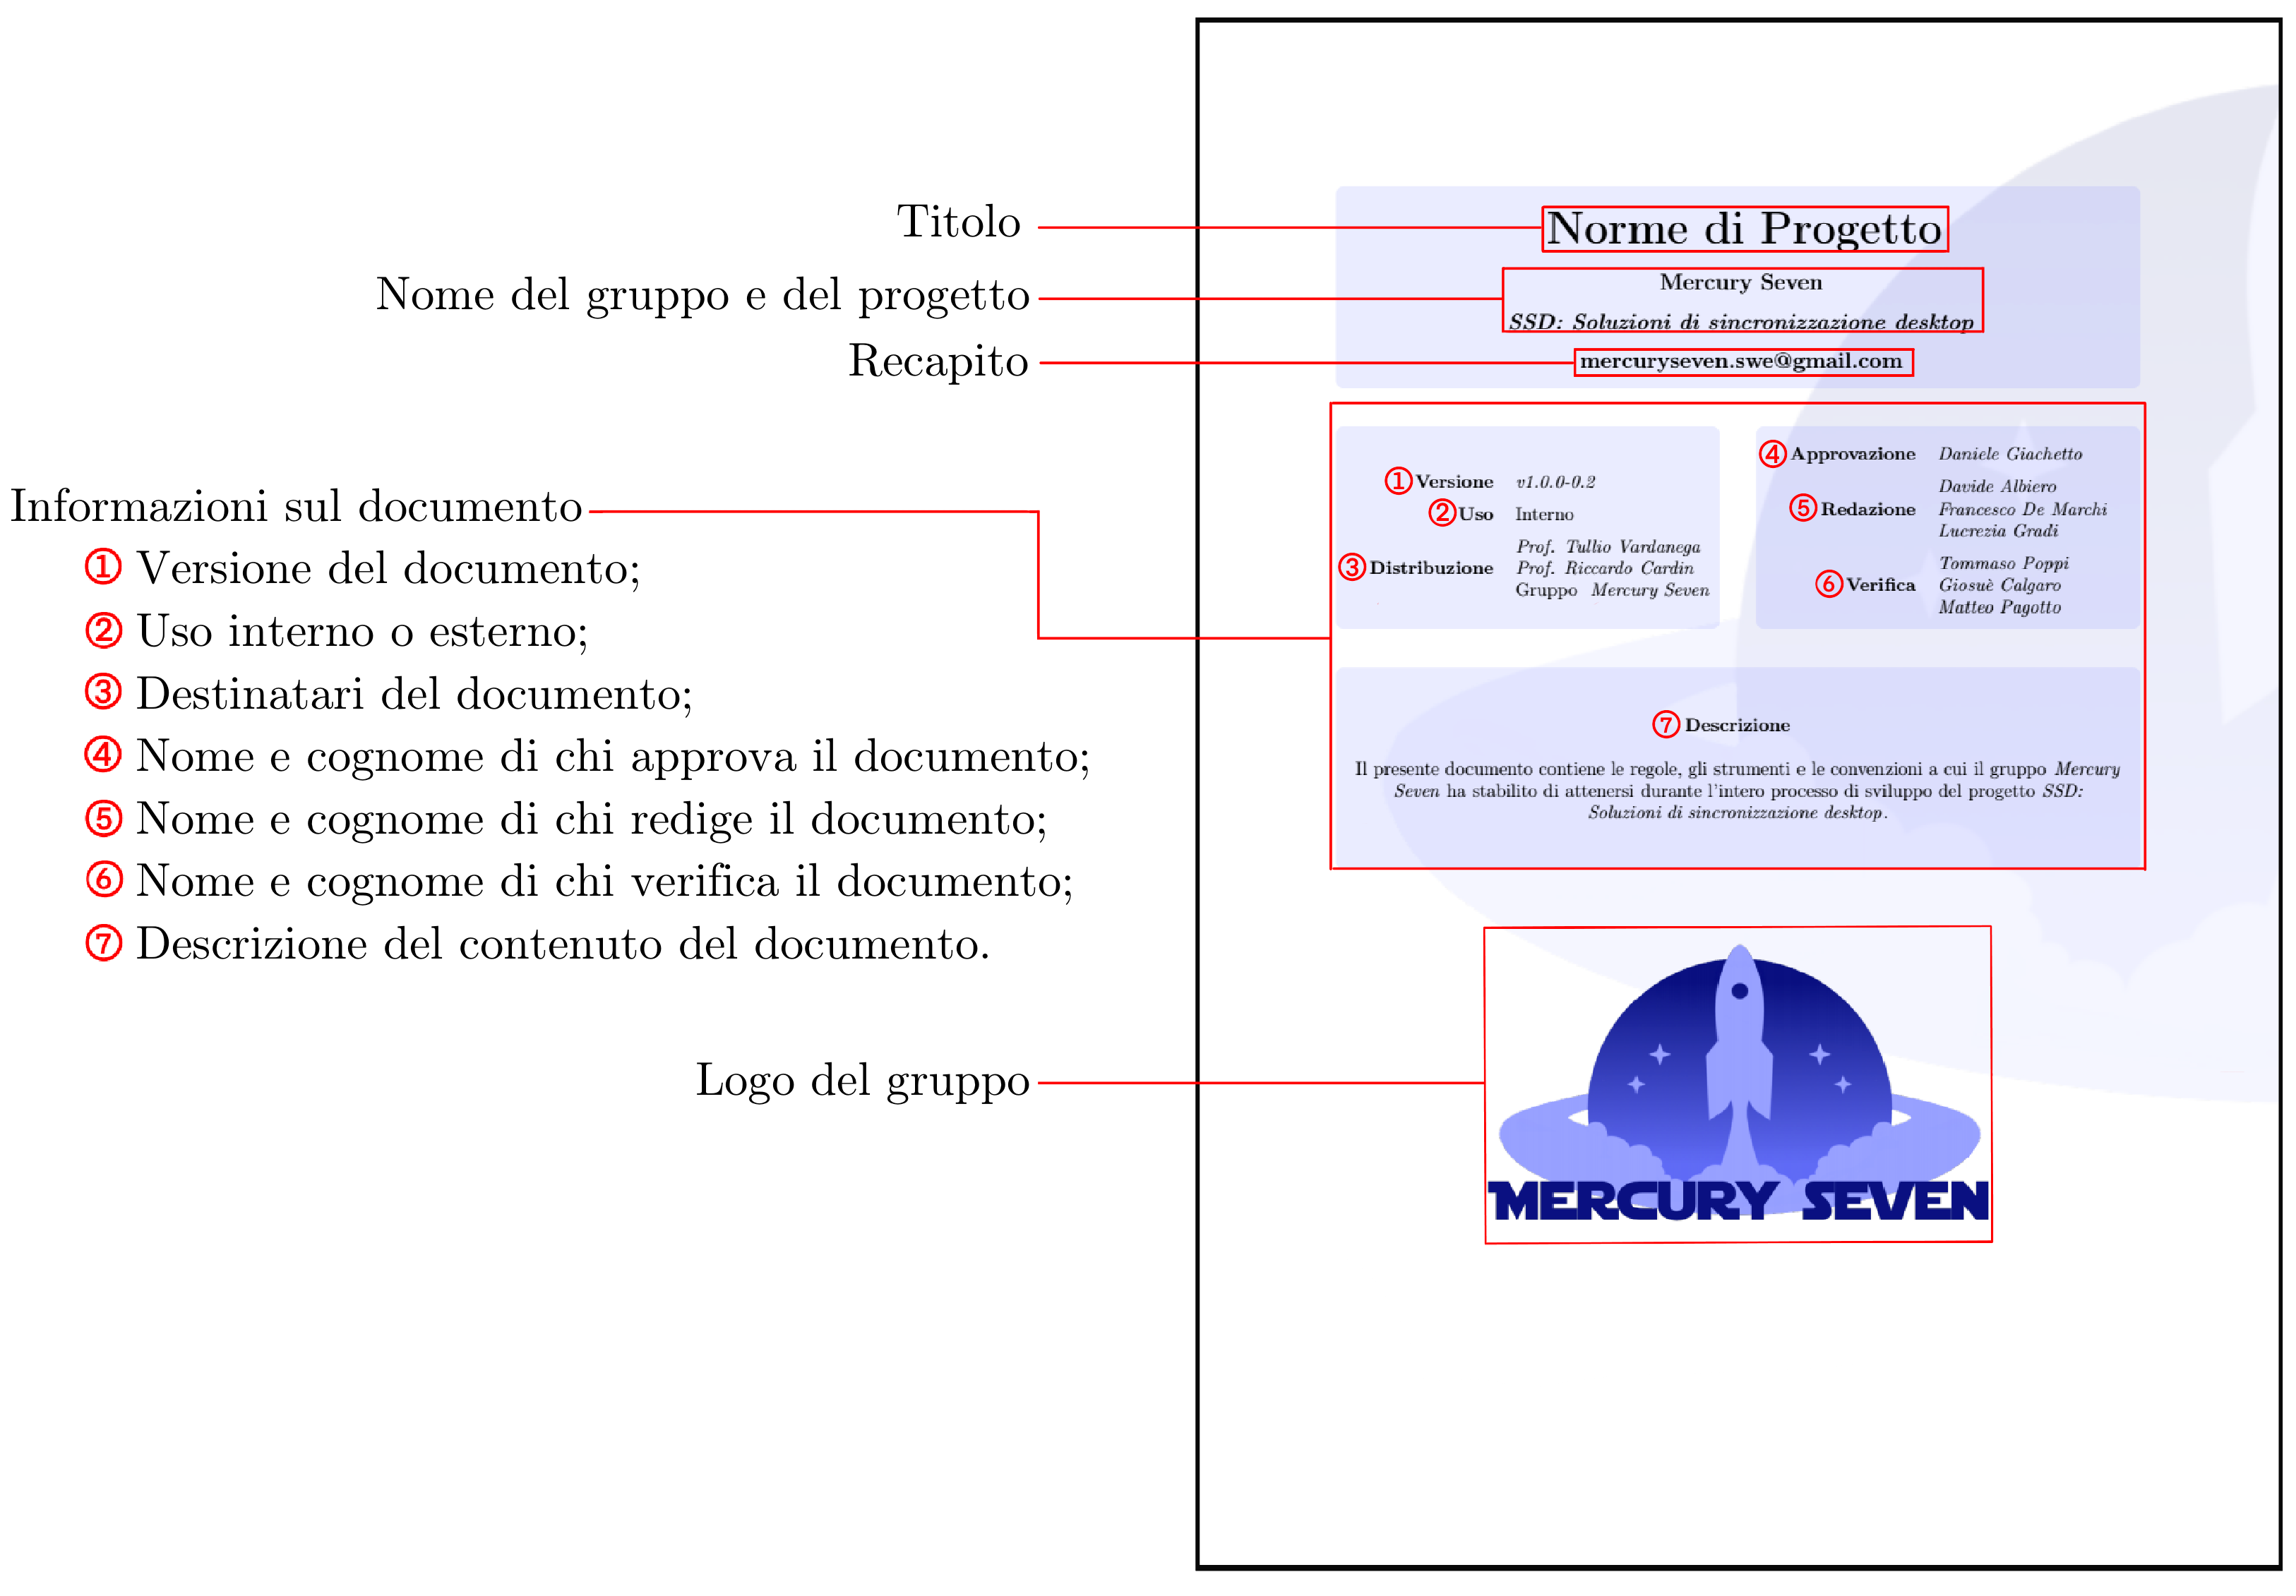
\includegraphics[scale = 0.6]{components/immagini/frontespizio.png}
    \caption{Struttura frontespizio}
\end{figure}


\paragraph*{Registro delle modifiche}      
Ogni documento presenta subito dopo il frontespizio il registro modifiche, esso è una tabella che traccia tutte le modifiche significative apportate al documento durante il suo ciclo di vita. Ogni voce della tabella riporta:

	\setlength{\freewidth}{\dimexpr\textwidth-1\tabcolsep}
	\renewcommand{\arraystretch}{1.5}
	\setlength{\aboverulesep}{0pt}
	\setlength{\belowrulesep}{0pt}
	\rowcolors{2}{AzzurroGruppo!10}{white}
	\begin{longtable}{L{.210\freewidth} L{.6\freewidth} L{.080\freewidth}}
		\rowcolor{AzzurroGruppo!30}
		\textbf{Nome} & \textbf{Descrizione} \\
		\toprule
		\endhead		
		
	\textbf{Versione} & Numero versione documento dopo la modifica \\
	\textbf{Data} & Data in cui è stata effettuata la modifica \\
	\textbf{Autore} & Nome e cognome dell'autore della modifica \\
	\textbf{Ruolo} & Ruolo dell'autore che ha apportato la modifica \\
	\textbf{Descrizione} & Sintetica descrizione delle modifiche apportate \\	
		
		\bottomrule
		\hiderowcolors
		\caption{Struttura registro delle modifiche}
	\end{longtable}


\paragraph*{Corpo del documento}       

\begin{figure}[H]
    \centering
    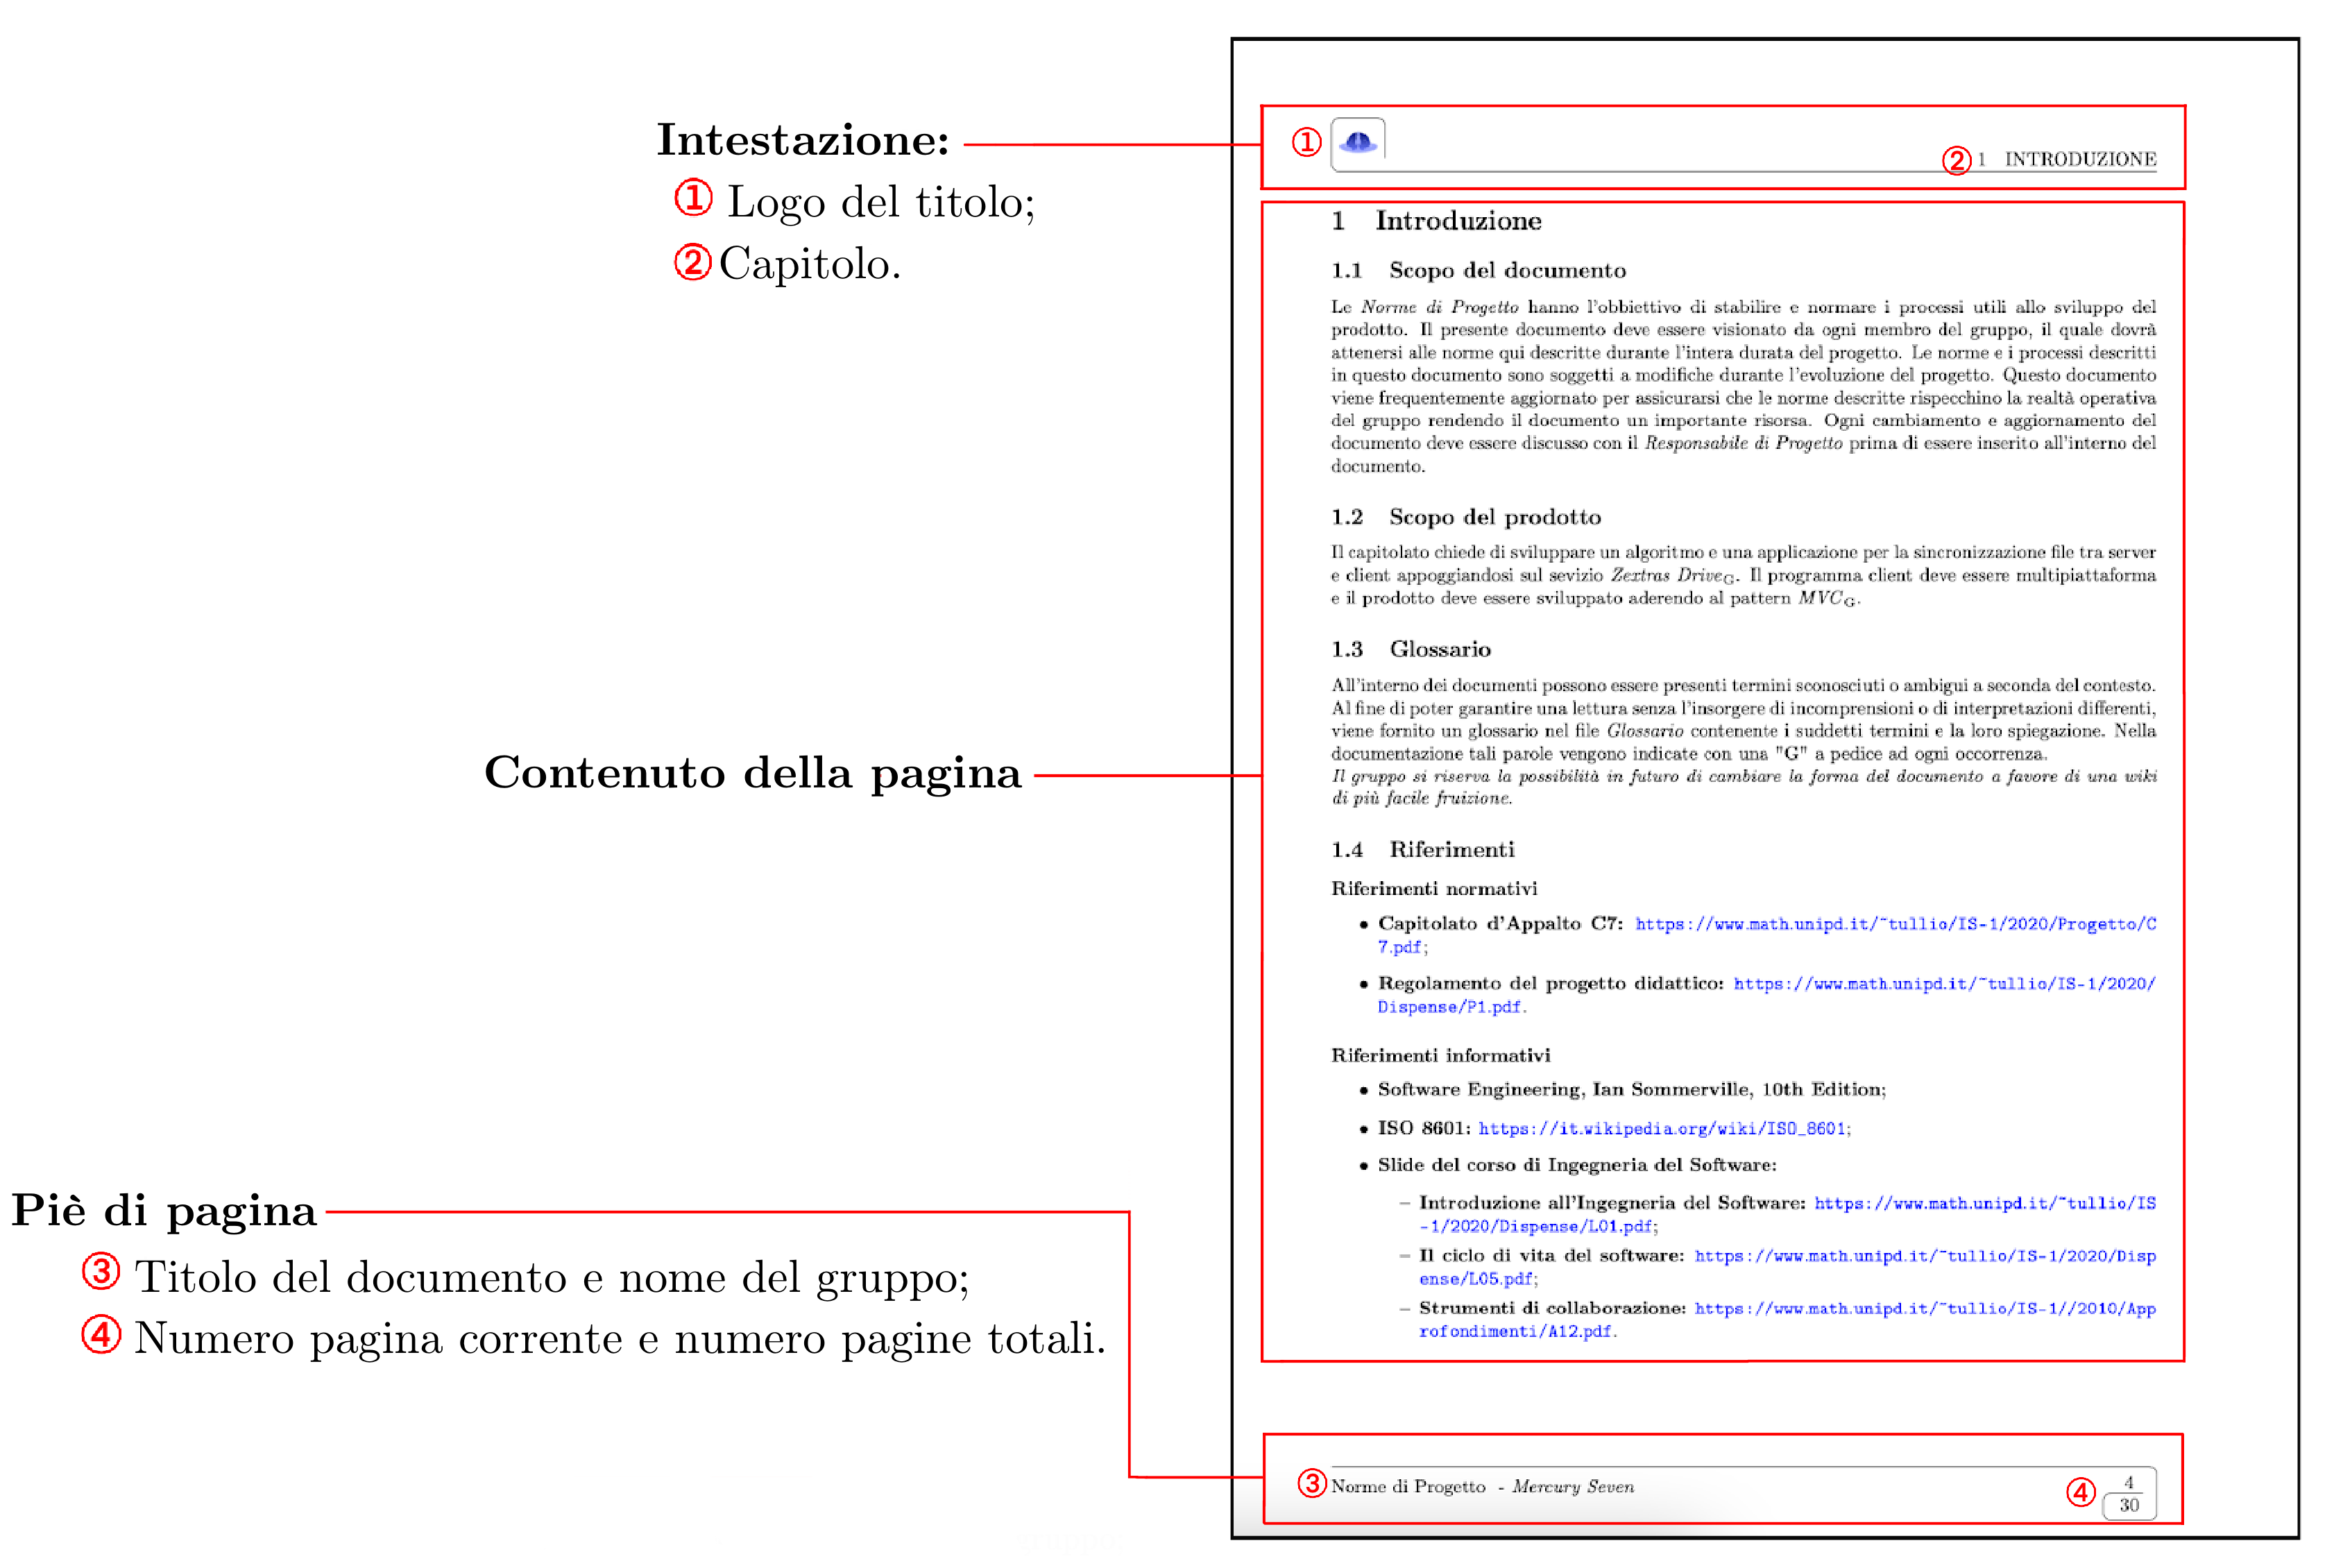
\includegraphics[scale = 0.6]{components/immagini/corpodocumento.png}
    \caption{Struttura corpo del documento}
\end{figure}


\paragraph*{Verbali}      
I verbali, sia interni che esterni, presentano una struttura fissa e sono soggetti alle stesse norme strutturali degli altri argomenti, ad eccezione del fatto che, essendo informali, non sono soggetti a versionamento.
La struttura sarà quindi la seguente:

	\setlength{\freewidth}{\dimexpr\textwidth-1\tabcolsep}
	\renewcommand{\arraystretch}{1.5}
	\setlength{\aboverulesep}{0pt}
	\setlength{\belowrulesep}{0pt}
	\rowcolors{2}{AzzurroGruppo!10}{white}
	\begin{longtable}{L{.210\freewidth} L{.6\freewidth} L{.080\freewidth}}
		\rowcolor{AzzurroGruppo!30}
		\textbf{Nome} & \textbf{Descrizione} \\
		\toprule
		\endhead		
		\textbf{Data} & Riporta la data della riunione \\
		\textbf{Ora inizio} & Riporta l'orario di inizio della riunione\\
		
		\textbf{Ora fine} & Riporta l'orario di fine della riunione \\
		\textbf{Segretario} & Nome e cognome dell'incaricato alla stesura del verbale \\
		\textbf{Partecipanti} & Contiene l'elenco dei presenti all'incontro \\  
		\textbf{Ordine del giorno} & Contiene l'elenco degli argomenti trattati durante la riunione \\
		\textbf{Resoconto} & Riporta l'esito della discussione dei singoli punti inseriti nell'ordine del giorno; per i verbali esterni, questa sezione è organizzata secondo il pattern domanda-risposta \\
		\textbf{Riepilogo delle decisioni} & Contiene una tabella che riassume tutte le decisioni avvenute durante la riunione, numerandole con un codice univoco del tipo: 
	\centerline{\textbf{V[Interno/Esterno]\_[YYYY]\_[MM]\_[DD].[X]}} con \textbf{X} indicante il numero progressivo della decisione, a partire da 1 \\		
		
		\bottomrule
		\hiderowcolors
		\caption{Descrizione struttura verbali}
	\end{longtable}


\subsubsection{Norme tipografiche}
\paragraph*{Convenzioni di denominazione}   
I nomi delle cartelle e dei file relativi ai documenti adottano la convenzione \glo{PascalCase}, ossia il nome del file presenta l'iniziale di ogni parola che lo compone in maiuscolo, senza nessun separatore. Per file e cartelle legati alla struttura del documento i nomi non contengono caratteri maiuscoli. 
\paragraph*{Stili di testo} 


	\setlength{\freewidth}{\dimexpr\textwidth-1\tabcolsep}
	\renewcommand{\arraystretch}{1.5}
	\setlength{\aboverulesep}{0pt}
	\setlength{\belowrulesep}{0pt}
	\rowcolors{2}{AzzurroGruppo!10}{white}
	\begin{longtable}{L{.210\freewidth} L{.6\freewidth} L{.080\freewidth}}
		\rowcolor{AzzurroGruppo!30}
		\textbf{Nome} & \textbf{Descrizione} \\
		\toprule
		\endhead		
		\textbf{Grassetto} & Viene usato nei titoli delle sezioni e dei paragrafi, per enfatizzare parole, per indicare gli elementi di un elenco puntato \\
		\textbf{Corsivo} & Viene usato per i nomi propri (membri del gruppo,  \glo{proponente} e committenti), per citare il nome di un documento e per i termini che fanno parte del glossario\\
		\textbf{Monospace} & Viene usato per gli snippet di codice \\
		\textbf{Maiuscolo} & Viene usato negli acronimi e, nel caso di nomi di documenti, per le lettere iniziali delle parole che li compongono secondo la convenzione \textit{\glo{PascalCase}} \\
		\bottomrule
		\hiderowcolors
		\caption{Descrizione stili di testo}
	\end{longtable}
\paragraph*{Glossario}  
Al fine di evitare ambiguità fra i termini è stato realizzato un documento denominato \textit{Glossario}. I termini il cui significato può risultare ambiguo saranno contrassegnati con una \textbf{G} a pedice (e.g: \texorpdfstring{glossario\textsubscript{\textbf{G}}})) ad ogni loro occorrenza e saranno riportati in ordine alfabetico con le loro rispettive definizioni. 
\paragraph*{Elenchi puntati}
\
{
	\setlength{\freewidth}{\dimexpr\textwidth-0\tabcolsep}
	\renewcommand{\arraystretch}{1.5}
	\setlength{\aboverulesep}{0pt}
	\setlength{\belowrulesep}{0pt}
	\rowcolors{2}{AzzurroGruppo!10}{white}
	\begin{longtable}{L{.25\freewidth} L{.75\freewidth}}
		\rowcolor{AzzurroGruppo!30}
		\textbf{Simbolo} & \textbf{Uso e descrizione} \\
		\toprule
		\endhead		
		\textbf{• (pallino)} & Simbolo per scandire il primo livello di annidamento degli elenchi puntati. \\ 
		\textbf{-- (doppio trattino)} & Simbolo per scandire il secondo livello di annidamento degli elenchi puntati.  \\
		\textbf{. (punto fermo)} & Simbolo per scandire il terzo livello di annidamento degli elenchi puntati. Inoltre viene utilizzato al termine dell'ultima voce di un elenco puntato \\
		\textbf{; (punto e virgola)} & Simbolo utilizzato al termine di ogni voce degli elenchi puntati salvo l'ultima\\
		\bottomrule
		\hiderowcolors
		\caption{Descrizione delle convenzioni usate negli elenchi puntati}
\end{longtable}
}
Ogni voce contenuta all'interno degli elenchi puntati inizia con la lettera maiuscola. Le voci che corrispondono allo schema NomeElemento-descrizione presentano il primo termine in grassetto, il secondo invece nel formato normale.
Gli elenchi puntati dovranno essere usati solo quando necessario, preferendo le tabelle ad essi quando possibile.
\paragraph*{Formato data e ora} 
Le date vengono indicato usato il formato stabilito dallo standard ISO 8601:\newline
\centerline{\textbf{[YYYY]\-[MM]\-[DD]}}
\newline

\
{
	\setlength{\freewidth}{\dimexpr\textwidth-0\tabcolsep}
	\renewcommand{\arraystretch}{1.5}
	\setlength{\aboverulesep}{0pt}
	\setlength{\belowrulesep}{0pt}
	\rowcolors{2}{AzzurroGruppo!10}{white}
	\begin{longtable}{L{.15\freewidth} L{.25\freewidth} L{.080\freewidth}}
		\rowcolor{AzzurroGruppo!30}
		\textbf{Sigla} & \textbf{Descrizione} \\
		\toprule
		\endhead		
		\textbf{[YYYY]} & Indica l'anno \\ 
		\textbf{[MM]} & Indica il mese  \\
		\textbf{[GG]} & Indica il giorno \\
		\bottomrule
		\hiderowcolors
		\caption{Descrizione delle sigle indicanti la data}
\end{longtable}
\paragraph*{Sigle}
Le seguenti tabelle riassumono tutte le sigle utilizzate e la loro descrizione. Le tabelle sono divise per argomento.
	\setlength{\freewidth}{\dimexpr\textwidth-1\tabcolsep}
	\renewcommand{\arraystretch}{1.5}
	\setlength{\aboverulesep}{0pt}
	\setlength{\belowrulesep}{0pt}
	\rowcolors{2}{AzzurroGruppo!10}{white}
	\begin{longtable}{L{.1\freewidth} L{.25\freewidth} L{.080\freewidth}}
		\rowcolor{AzzurroGruppo!30}
		\textbf{Sigla} & \textbf{Nome} \\
		\toprule
		\endhead		
		 \textbf{AdR}& Analisi dei \ignore{Requisiti} \\
		 \textbf{SdF} & Studio di Fattibilità \\
		 \textbf{NdP} & Norme di Progetto \\
		 \textbf{PdP} & Piano di Progetto \\
		 \textbf{PdQ} & Piano di Qualifica \\
		 \textbf{G} & Glossario \\
		 \textbf{VE} & Verbale Esterno \\
		 \textbf{VI} & Verbale Interno \\

		\bottomrule
		\hiderowcolors
		\caption{Sigle relative ai nomi dei documenti}
	\end{longtable}
	\newpage{}
	\setlength{\freewidth}{\dimexpr\textwidth-1\tabcolsep}
	\renewcommand{\arraystretch}{1.5}
	\setlength{\aboverulesep}{0pt}
	\setlength{\belowrulesep}{0pt}
	\rowcolors{2}{AzzurroGruppo!10}{white}
	\begin{longtable}{L{.1\freewidth} L{.25\freewidth} L{.080\freewidth}}
		\rowcolor{AzzurroGruppo!30}
		\textbf{Sigla} & \textbf{Nome} \\
		\toprule
		\endhead		
		 \textbf{RE}& Responsabile \\
		 \textbf{AM} & Amministratore \\
		 \textbf{AN} & Analista \\
		 \textbf{PR} & Progettista \\
		 \textbf{PT} & Programmatore \\
		 \textbf{VE} & Verificatore \\

		\bottomrule
		\hiderowcolors
		\caption{Sigle ruoli di progetto}
	\end{longtable}
		
		\setlength{\freewidth}{\dimexpr\textwidth-1\tabcolsep}
	\renewcommand{\arraystretch}{1.5}
	\setlength{\aboverulesep}{0pt}
	\setlength{\belowrulesep}{0pt}
	\rowcolors{2}{AzzurroGruppo!10}{white}
	\begin{longtable}{L{.1\freewidth} L{.3\freewidth} L{.080\freewidth}}
		\rowcolor{AzzurroGruppo!30}
		\textbf{Sigla} & \textbf{Nome} \\
		\toprule
		\endhead		
		 \textbf{RR}& Revisione dei \ignore{requisiti} \\
		 \textbf{RP} & Revisione di Progettazione \\
		 \textbf{RQ} & Revisione di Qualifica \\
		 \textbf{RA} & Revisione di Accettazione \\
		 

		\bottomrule
		\hiderowcolors
		\caption{Sigle relative alle revisioni di progetto}
	\end{longtable}	
\subsubsection{Elementi grafici}

	\setlength{\freewidth}{\dimexpr\textwidth-1\tabcolsep}
	\renewcommand{\arraystretch}{1.5}
	\setlength{\aboverulesep}{0pt}
	\setlength{\belowrulesep}{0pt}
	\rowcolors{2}{AzzurroGruppo!10}{white}
	\begin{longtable}{L{.2\freewidth} L{.6\freewidth} L{.080\freewidth}}
		\rowcolor{AzzurroGruppo!30}
		\textbf{Nome} & \textbf{Descrizione} \\
		\toprule
		\endhead		
		 \textbf{Immagini} & Le figure saranno centrate ed avranno una opportuna didascalia \\
		  \textbf{Grafici UML} & I grafici in linguaggio UML saranno inseriti nel documento come immagini \\
		  \textbf{Tabelle} & Ogni tabella è contrassegnata da una didascalia e numerata in modo progressivo. Fanno eccezione le tabelle del registro delle modifiche, che non presentano una didascalia \\
		 

		\bottomrule
		\hiderowcolors
		\caption{Descrizione elementi grafici}
	\end{longtable}	

\subsubsection{Metriche}

{
	\setlength{\freewidth}{\dimexpr\textwidth-0\tabcolsep}
	\renewcommand{\arraystretch}{1.5}
	\setlength{\aboverulesep}{0pt}
	\setlength{\belowrulesep}{0pt}
	\rowcolors{2}{AzzurroGruppo!10}{white}
	\begin{longtable}{L{.1\freewidth} L{.15\freewidth} L{.3\freewidth} L{.35\freewidth}}
		\rowcolor{AzzurroGruppo!30}
		\textbf{Codice} & \textbf{Nome} & \textbf{Descrizione metrica} & \textbf{Formula/Valore}\\
		\toprule
		\endhead		
		\textbf{MDC01} & Indice di Gulpease & Indice che riporta il grado di leggibilità di un testo redatto in lingua italiana & \small{$Ig= 89 + \frac{300 * (n\ frasi) - 10 * (n\ lettere)}{n\ parole}$} \\
		\textbf{MDC02} & Correttezza Ortografica & Indice che riporta la correttezza ortografica del testo. Questo valore deve essere il più elevato possibile come indicato nel \PdQ{} & Correttezza >= 95\% \\
		
		\bottomrule
		\hiderowcolors
		\caption{Descrizione delle metriche}\\
	\end{longtable}
}


\subsubsection{Strumenti di stesura}

	\setlength{\freewidth}{\dimexpr\textwidth-1\tabcolsep}
	\renewcommand{\arraystretch}{1.5}
	\setlength{\aboverulesep}{0pt}
	\setlength{\belowrulesep}{0pt}
	\rowcolors{2}{AzzurroGruppo!10}{white}
	\begin{longtable}{L{.210\freewidth} L{.75\freewidth} L{.080\freewidth}}
		\rowcolor{AzzurroGruppo!30}
		\textbf{Nome} & \textbf{Descrizione} \\
		\toprule
		\endhead		
		\textbf{\LaTeX} & Linguaggio compilato che permette un facile versionamento, la produzione coerente, ordinata, templetizzata e collaborativa dei documenti \\
		\textbf{Texmaker} & Editor intuitivo che permette una facile compilazione e visualizzazione dei documenti. \newline \url{(https://www.xm1math.net/texmaker/)}\\
		\bottomrule
		\hiderowcolors
		\caption{Strumenti utilizzati durante il processo di documentazione}
	\end{longtable}

\subsection{Gestione della configurazione}
Il processo di gestione della configurazione ha come scopo il gestire in maniera ordinata e sistematica la produzione di documenti e codice. In particolare, un elemento sottoposto a configurazione ha una collocazione, una denominazione e uno stato definiti, oltre che avere garantite modifica normata e versionamento. Le attività coinvolte sono:
\begin{enumerate}
	\item implementazione del processo;
	\item identificazione della configurazione;
	\item controllo della configurazione;
	\item resoconto dello stato della configurazione (gestione delle modifiche);
	\item valutazione della configurazione;
	\item gestione del rilascio e consegna.
\end{enumerate}
\subsubsection{Versionamento}
\paragraph*{Codice di versionamento}
\label{cod-versionamento}
La storia di un prodotto realizzato dal gruppo, che questo sia un documento o codice, deve poter essere sempre ricostruibile attraverso le sue versioni. Il codice di una versione è nel formato\newline
\centerline{\textbf{[X].[Y].[Z]-[a].[b]}}\newline{}
\newpage{}
\setlength{\freewidth}{\dimexpr\textwidth-0\tabcolsep}
	\renewcommand{\arraystretch}{1.5}
	\setlength{\aboverulesep}{0pt}
	\setlength{\belowrulesep}{0pt}
	\rowcolors{2}{AzzurroGruppo!10}{white}
	\begin{longtable}{L{.210\freewidth} L{.6\freewidth} L{.080\freewidth}}
		\rowcolor{AzzurroGruppo!30}
		\textbf{Sigla} & \textbf{Descrizione} \\
		\toprule
		\endhead
		\textbf{[X]} & Indica il numero incrementale di revisione del responsabile di progetto. \\
		\textbf{[Y]} & Indica il numero incrementale della \glo{verifica}. \\
		\textbf{[Z]} & Indica il numero di modifiche apportate al documento, che riparte da 0 dopo ogni \glo{verifica} ed approvazione. \\
		\textbf{[a]} & Indica una versione completa e funzionante del prodotto: le componenti \glo{software} implementano tutti i \glo{requisiti} obbligatori, i \glo{test} sono stati tutti superati, le \glo{metriche} di qualità soddisfatte e sono presenti versioni approvate di tutti i documenti richiesti per il prodotto finale. Viene incrementato quando il prodotto \glo{software} non è più retrocompatibile; la numerazione parte da 0 e non viene annullata. \\
		\textbf{[b]} & Indica un incremento nello sviluppo totale del prodotto: la numerazione incrementa ad ogni \glo{sprint}, partendo da 1 e non venendo mai annullata. \\
		\bottomrule
		\hiderowcolors
		\caption{Descrizione codice di versionamento}
	\end{longtable}
Ogni incremento deve essere associato ad una \glo{verifica} delle modifiche apportate.\newline{}
Le modifiche apportate in attesa di \glo{verifica} vengono identificate con un codice numerico progressivo che riparte da 0 ad ogni \glo{verifica}.
\paragraph*{Tecnologie adottate}
Per la gestione delle versioni è stato scelto di utilizzare il \glo{sistema} di versionamento distribuito \textit{\glo{Git}} con due \glo{repository} remoti presenti su \textit{\glo{GitHub}}.
\paragraph*{Repository}
Il gruppo \textit{\Gruppo{}} ha scelto di creare due \glo{repository} per il progetto:
\begin{itemize}
	\item \textbf{project-SSD} per il versionamento del codice realizzato(\url{https://github.com/MercurySeven/project-SSD});
	\item \textbf{\repoDoc{}} per il versionamento dei documenti redatti (\url{https://github.com/MercurySeven/project-docs}).
\end{itemize}
Il gruppo ha deciso di optare per una separazione logica del codice e della documentazione per poter avere una struttura ed una organizzazione migliore. I due repository sono comunque entrambi facilmente reperibili nella pagina dell'organizzazione (\url{https://github.com/MercurySeven}).
\paragraph*{Struttura del repository}
Per entrambi i \glo{repository}, esiste una versione \textbf{locale} sul computer di ogni membro ed una versione \textbf{remota} su \textit{\glo{GitHub}}.\newline
Il \glo{repository} \textbf{project-SSD} è strutturato nel seguente modo:
\begin{itemize}
	\item \textbf{docs:} cartella contenente guide per installazione ed utilizzo del prodotto;
	\item \textbf{src:} cartella contenente il codice;
	\item \textbf{tests:} cartella contenente i \glo{test} del codice;
\end{itemize}
Il \glo{repository} \textbf{\repoDoc{}} è invece strutturato nel seguente modo:
\begin{itemize}
	\item \textbf{Tutorial:} cartella contenente un esempio di documento \LaTeX che elenca anche le basi del linguaggio e del suo utilizzo; 
	\item \textbf{Stile:} cartella contenente i file del template in linguaggio \LaTeX usato per produrre tutti i documenti;
	\item Una cartella per ogni documento prodotto.
\end{itemize}
Si è optato per questa soluzione per poter avere una documentazione in continua evoluzione, senza categorizzarla e bloccarla negli stati delle revisioni tramite sottocartelle contenenti le versioni delle documentazioni durante una specifica revisione.
\paragraph*{Tipi di file}
Nelle singole cartelle dei documenti sono inclusi:
\begin{itemize}
\item file \textit{README.md};
\item file \textit{.tex} per i sorgenti in \LaTeX; 
\item file \textit{.png} per le immagini da inserire nei documenti.
\end{itemize}
Il file \textit{.gitignore} contiene al suo interno un riferimento a tutti i file che non verranno versionati; il file è posizionato al livello più esterno del \glo{repository}.
\paragraph*{Norme di branching}
\label{NormeBranching}
Il \glo{repository} inerente alla documentazione sarà composto da diversi \glo{branch}:
\begin{itemize}
	\item \textbf{Main:} \glo{branch} principale che viene aggiornato solamente quando un documento arriva in fase di rilascio, essa avviene quando incrementa la \textbf{[X]} di una versione del documento (\S{}\ref{cod-versionamento});
	\item un \glo{branch} per ogni documento, usato per le modifiche minori effettuate tra i vari rilasci. Una volta che un documento ha raggiunto una maturità sufficiente per un rilascio, verrà eseguito una operazione di \glo{merge} con il \textbf{main}.
\end{itemize}
\paragraph*{Modifiche ai repository}
Tutti i membri del gruppo possono apportare modifiche ai file elaborati, salvo quelli presenti nel ramo \textbf{main}. Per apportare cambiamenti a questo ramo, come già citato in precedenza (\S{}\ref{NormeBranching}), è necessaria una \textit{pull request}, con conseguente approvazione di \textbf{almeno} un altro elemento del gruppo.\newline
Per modifiche minori ai file ogni singolo membro può operare con libero arbitrio, mentre per modifiche più sostanziose deve essere contattato il \RdP{} per il file in questione.\newline
Ogni modifica deve poter essere giustificata davanti a tutto il \glo{team}.
\newpage
\subsection{Accertamento della qualità}

Il processo di accertamento della qualità ha lo scopo di garantire la qualità del prodotto finale, cioè che rispetti i \glo{requisiti} di qualità individuati dagli \glo{stakeholder} e che le esigenze espresse dal \glo{proponente} vengano soddisfatte. Le strategie di sviluppo e gli standard adottati per assicurare la qualità della documentazione e del prodotto vengono formalizzati nel \PdQ{}, documento che fissa i \glo{requisiti} qualitativi e le \glo{metriche} relative ai processi impiegati e ai prodotti sviluppati. Quest'ultimo viene costantemente aggiornato per tenere traccia di eventuali cambiamenti ed è strutturato in modo tale da distinguere la parte riguardante la documentazione e quella riguardante il \glo{software}.
\subsubsection{Controllo di qualità}
Il gruppo \textit{\Gruppo{}} ritiene fondamentale stabilire delle regole che tutti i membri vadano a rispettare per il pieno raggiungimento di un \glo{sistema} di qualità predisposto al miglioramento continuo.
Le attività che ciascun membro deve svolgere sono:
\begin{itemize}
	\item comprensione degli obiettivi da raggiungere;
	\item individuazione di errori e discrepanze;
	\item produzione di una stima del valori di ogni task;
	\item produzione di una stima della complessità di ogni task;
	\item impiego delle conoscenze di ciascun membro del gruppo;
	\item produzione di risultati concreti nel tempo stimato;
	\item miglioramento continuo della propria formazione;
	\item continua comunicazione con il gruppo;
	\item rispetto totale degli standard e delle normative presenti all'interno del suddetto documento.
\end{itemize} 
\subsubsection{Denominazione delle metriche}
Per la denominazione delle \glo{metriche} il gruppo ha deciso di adottare il formato\newline \centerline{\textbf{M[Processo/Attività][Numero]}}\newline
dove
\begin{itemize}
	\item \textbf{M} indica che ci si sta riferendo ad una metrica;
	\item \textbf{Processo/Attività}: specifica il processo o l'attività tra:
	\begin{itemize}
		\item AR: \AdR{};
		\item PR: \emph{Progettazione};
		\item CD: \emph{Codifica};
		\item DC: \emph{Documentazione};
		\item VR: \emph{\glo{Verifica}};
		\item VL: \emph{\glo{Validazione}}.
	\end{itemize}
	\item \textbf{Numero}: definisce il codice univoco della metrica.
\end{itemize}
\subsubsection{Istanziazione di un processo}
Con il perseguimento della qualità in mente, il gruppo \textit{\Gruppo{}} ha deciso di adottare le seguenti regole al momento della definizione di ogni processo, in modo da curare la qualità sin dall'istanziazione dei processi:
\begin{itemize}
	\item un singolo processo deve essere più atomico possibile;
	\item l'obiettivo di un processo non può entrare in conflitto con quello di altri processi;
	\item l'affidamento di risorse umane, temporali e materiali ai singoli processi deve tenere conto tutti gli altri processi e deve puntare ad essere più efficiente possibile;
	\item ogni processo deve essere pianificato correttamente tramite una opportuna analisi dei rischi;
	\item ogni processo al termine della pianificazione deve avere una durata ben definita.
\end{itemize}
\subsection{Verifica}
Il processo di \glo{verifica} si occupa di determinare se i prodotti di una data attività sono corretti, coesi e completi e di individuare eventuali errori introdotti nella fase di sviluppo. Si compone di due attività che permettono di verificare che il prodotto sia conforme alle aspettative di analisi e di \glo{test} (\S{}\ref{veractivity}); per questo, il corretto funzionamento del processo è garantito dal rispetto delle seguenti regole: 
\begin{itemize}
	\item seguire procedure definite;
	\item seguire criteri chiari ed affidabili;
	\item passaggio del prodotto attraverso fasi successive opportunamente verificate;
	\item il prodotto deve trovarsi in uno stato stabile dopo la \glo{verifica};
	\item alla fine del processo deve essere possibile procedere alla fase di \glo{validazione}.
\end{itemize}
Sono soggetti a \glo{verifica} sia il \glo{software} che la documentazione. 

\subsubsection{Attività} \label{veractivity}

\setlength{\freewidth}{\dimexpr\textwidth-0\tabcolsep}
	\renewcommand{\arraystretch}{1.5}
	\setlength{\aboverulesep}{0pt}
	\setlength{\belowrulesep}{0pt}
	\rowcolors{2}{AzzurroGruppo!10}{white}
	\begin{longtable}{L{.15\freewidth} L{0.35\freewidth} L{0.5\freewidth}}
		\rowcolor{AzzurroGruppo!30}
		\textbf{Nome} & \textbf{Descrizione} & \textbf{Attuazione} \\
		\toprule
		\endhead	
		\multirow{2}{.15\freewidth}{\textbf{Analisi statica}}
		 & \multirow{2}{0.35\freewidth}{L'analisi statica permette di effettuare controlli su documenti e codice, verificando così che la corretta applicazione della correttezza (intesa come assenza di errori e difetti).}&\textbf{Walkthrough:} tecnica di \glo{verifica} consistente nella lettura da parte del \glo{team} dell'intero documento o codice in cerca di anomalie. Verrà applicata principalmente nella fase iniziale del progetto, quando il \glo{team} ancora non conosce i possibili errori che si possono incontrare. Questa tecnica risulta molto onerosa in termini di efficienza ed efficacia. \\
		 \cline{3-3} 
		 & & \textbf{Inspection:} tecnica di \glo{verifica} attraverso il quale il \textit{Verificatore} eseguirà una lettura mirata e strutturata del documento o del codice nei punti in cui si sa già che possano essere presenti degli errori. Risulta meno dispendiosa in termini di tempo ma richiede una buona conoscenza di fondo. \\
		 \textbf{Analisi dinamica} & L'analisi dinamica prevede l'esecuzione del prodotto \glo{software} e la sua analisi tramite l'utilizzo di \glo{test} che verificano se il prodotto funziona o se vi sono presenti anomalie. & L'attività di testing è la base dell'analisi dinamica. I \glo{test} permettono di individuare tutti i possibili errori che possono essere stati commessi e tutti i casi limite che possono risultare problematici. I parametri da definire per ogni \glo{test} sono descritti nella seguente tabella. \\
		\bottomrule
		\hiderowcolors
		\caption{Descrizione della attività}
	\end{longtable}

I parametri da definire per ogni \glo{test} sono descritti nella seguente tabella.

\setlength{\freewidth}{\dimexpr\textwidth-0\tabcolsep}
	\renewcommand{\arraystretch}{1.5}
	\setlength{\aboverulesep}{0pt}
	\setlength{\belowrulesep}{0pt}
	\rowcolors{2}{AzzurroGruppo!10}{white}
	\begin{longtable}{L{.210\freewidth} L{.6\freewidth} L{.080\freewidth}}
		\rowcolor{AzzurroGruppo!30}
		\textbf{Nome} & \textbf{Descrizione} \\
		\toprule
		\endhead		
		\textbf{Ambiente} & \glo{Sistema} hardware e \glo{software} sulla quale viene eseguito il \glo{test} \\
		\textbf{Stato iniziale} & Stato iniziale dal quale parte il \glo{test} \\
		 \textbf{Input} & Tutti i dati ammessi in ingresso \\
		\textbf{Output} & Tutti i dati attesi in uscita \\
		 \textbf{Istruzioni aggiuntive} & Istruzioni opzionali che permettono di impostare come il \glo{test} deve essere eseguito e come i risultati devono essere interpretati \\
		\bottomrule
		\hiderowcolors
		\caption{Parametri dei test}
	\end{longtable}


Dei \glo{test} ben progettati e scritti devono:
\begin{itemize}
	\item essere ripetibili;
	\item definire correttamente ed identificare i parametri già elencati;
	\item avvertire la presenza di effetti indesiderati nel codice;
	\item fornire informazioni sui risultati e sull'esecuzione stessa tramite file di log.
\end{itemize}

\paragraph*{Codice identificativo dei test}
Ogni \glo{test} viene descritto con:
\begin{itemize}
	\item codice identificativo;
	\item requisito;
	\item descrizione;
	\item stato, che può essere:
	\begin{itemize}
		\item \textbf{I:} implementato;
		\item \textbf{NI:} non implementato;
		\item \textbf{NE:} non eseguito;
		\item \textbf{S:} superato;
		\item \textbf{NS:} non superato.
	\end{itemize}
\end{itemize}
Il codice identificativo presenta la seguente struttura:\newline
\centerline{\textbf{T[Tipo][Priorità][Id]}}
\newline
Dove:
\begin{itemize}
	\item \textbf{T:} indica il "\ignore{Test}";
	\item \textbf{Tipo:}
		\begin{itemize}
			\item \textbf{U:} \glo{test di \ignore{unità}};
			\item \textbf{I:} \glo{test di integrazione};
			\item \textbf{S:} \glo{test di \ignore{sistema}};
			\item \textbf{R:} \glo{test di regressione};
			\item \textbf{A:} \glo{test di accettazione};
		\end{itemize}
	\item \textbf{Priorità:}
		\begin{itemize}
			\item \textbf{O:} \ignore{test} obbligatorio;
			\item \textbf{D:} \ignore{test} desiderabile;
			\item \textbf{F:} \ignore{test} facoltativo;
		\end{itemize}
	\item \textbf{Id:} codice identificativo.
\end{itemize}

\subsubsection{Metriche}
Il gruppo ritiene prematuro stabilire in questa fase delle \glo{metriche} per i \glo{test} in questione. La sezione sarà opportunamente integrata.

\setlength{\freewidth}{\dimexpr\textwidth-0\tabcolsep}
	\renewcommand{\arraystretch}{1.5}
	\setlength{\aboverulesep}{0pt}
	\setlength{\belowrulesep}{0pt}
	\rowcolors{2}{AzzurroGruppo!10}{white}
	\begin{longtable}{L{.210\freewidth} L{.6\freewidth} L{.080\freewidth}}
		\rowcolor{AzzurroGruppo!30}
		\textbf{Nome} & \textbf{Descrizione} \\
		\toprule
		\endhead
		\textbf{\ignore{Verifica} ortografica} & Per la \glo{verifica} ortografica dei documenti scritti in \LaTeX si utilizzerà \glo{GNU aspell} ed il correttore automatico fornito da \glo{TexMaker} \\
		\bottomrule
		\hiderowcolors
		\caption{Metriche processo di verifica}
	\end{longtable}
\subsection{Validazione}
Il processo di \glo{validazione} stabilisce se il prodotto è in grado di soddisfare il compito per il quale è stato creato e se rispetta i \glo{requisiti} e le aspettative del committente. In particolare, prende in esame il prodotto ottenuto dalla fase di \glo{verifica} e lo restituisce garantendo che esso sia conforme ai \glo{requisiti} e ai bisogni del committente. Sarà compito del \RdP{} controllare i risultati e decidere se approvare o rigettare il documento, con conseguente richiesta di un nuovo processo. Sarà quindi fondamentale l'elaborazione di una strategia per rendere riutilizzabili le procedure di \glo{verifica}. 

